\documentclass{beamer}

\usepackage[utf8]{inputenc}
\usepackage{hyperref}

\usetheme{Berkeley}
\beamertemplatenavigationsymbolsempty
\setbeamertemplate{headline}{}
 
\title{Importing data into FoodChain-Lab 1}
\date{}
 
\begin{document}
\maketitle

\section{ }

\subsection{Tasks}
\begin{frame}
	\begin{itemize}
		\item In this tutorial we'll show you how to import delivery data to FoodChain-Lab via our Excel templates.
		\item We will first import the initial data for the outbreak locations and then successively add the delivery data for caterers and other suppliers via autogenerated back- and forward-tracing templates.
	\end{itemize}
\end{frame}
 
\subsection{1}
\begin{frame}
	\begin{center}
  		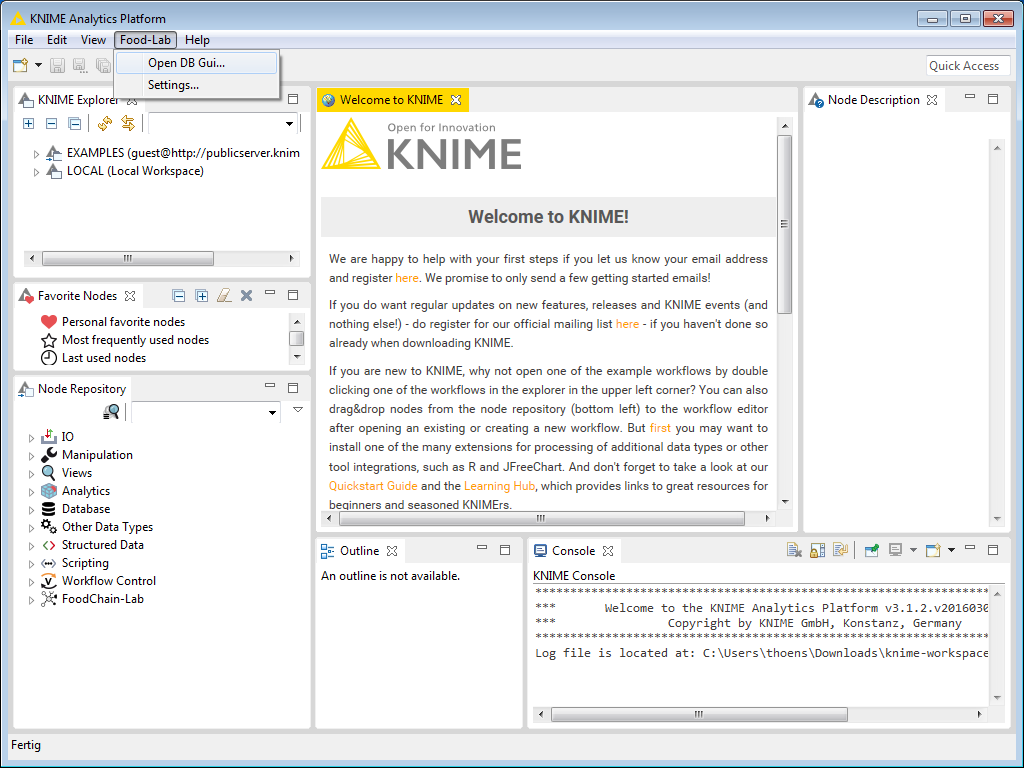
\includegraphics[height=0.6\textheight]{1.png}
	\end{center}
	\begin{itemize}
		\item Select \textbf{Food-Lab $>$ Open DB Gui...} in the menu bar to open the database interface.
	\end{itemize}
\end{frame}

\subsection{2}
\begin{frame}
	\begin{center}
  		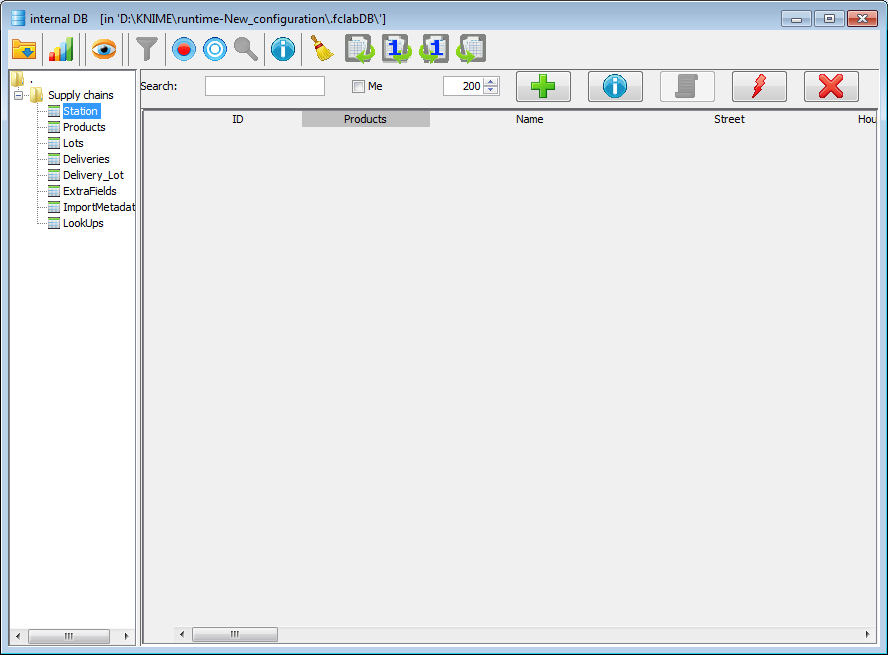
\includegraphics[height=0.35\textheight]{2.png}
	\end{center}
	\begin{itemize}
		\item The FoodChain-Lab database interface now pops up.
		\item Here you can import, edit and validate food delivery data.
		\item To start the data import you must download, fill out and import the "Start Tracing Backward" or  the "Start Tracing Forward" template.
		\item Backward: \url{https://github.com/SiLeBAT/BfROpenLabResources/raw/master/GitHubPages/templates/Start_Tracing_Backward.xlsx}.
		\item Forward: \url{https://github.com/SiLeBAT/BfROpenLabResources/raw/master/GitHubPages/templates/Start_Tracing_Forward.xlsx}.
	\end{itemize}
\end{frame}

\subsection{3}
\begin{frame}
	\begin{center}
  		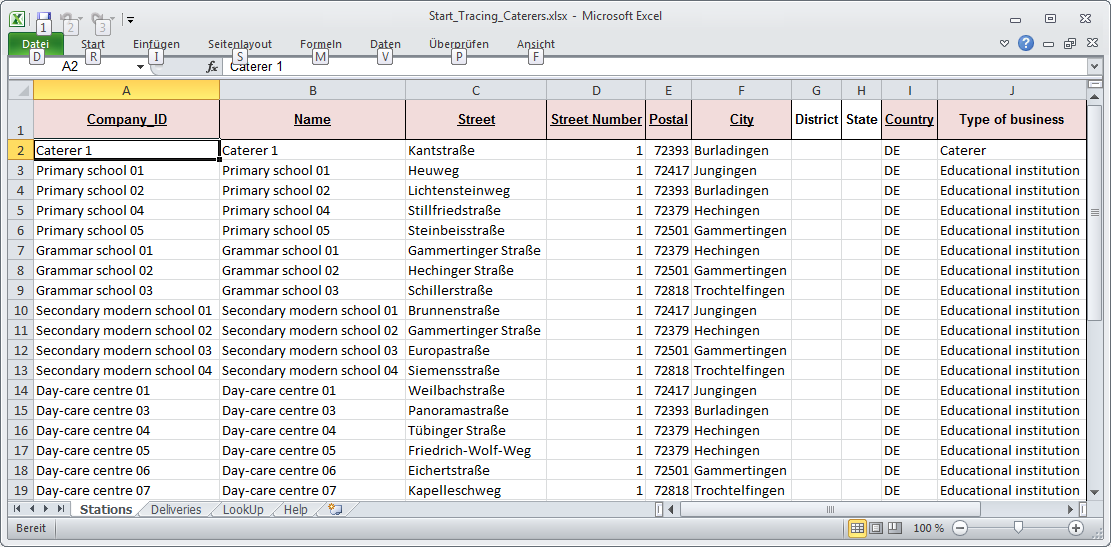
\includegraphics[height=0.5\textwidth]{3.png}
	\end{center}
	\begin{itemize}
		\item For this tutorial we have already pre-prepared "Start Tracing Forward" templates for two \textbf{Caterers}, at which some contaminated food products were detected.
		\item These templates contain deliveries from the \textbf{Caterers} to several \textbf{Educational Institutions}.
		\item Here we start with "Forward" instead of "Backward" templates, since we first want to know the recipients of the \textbf{Caterers'} menus and not the suppliers of the ingredients.
	\end{itemize}
\end{frame}

\subsection{4}
\begin{frame}
	\begin{center}
  		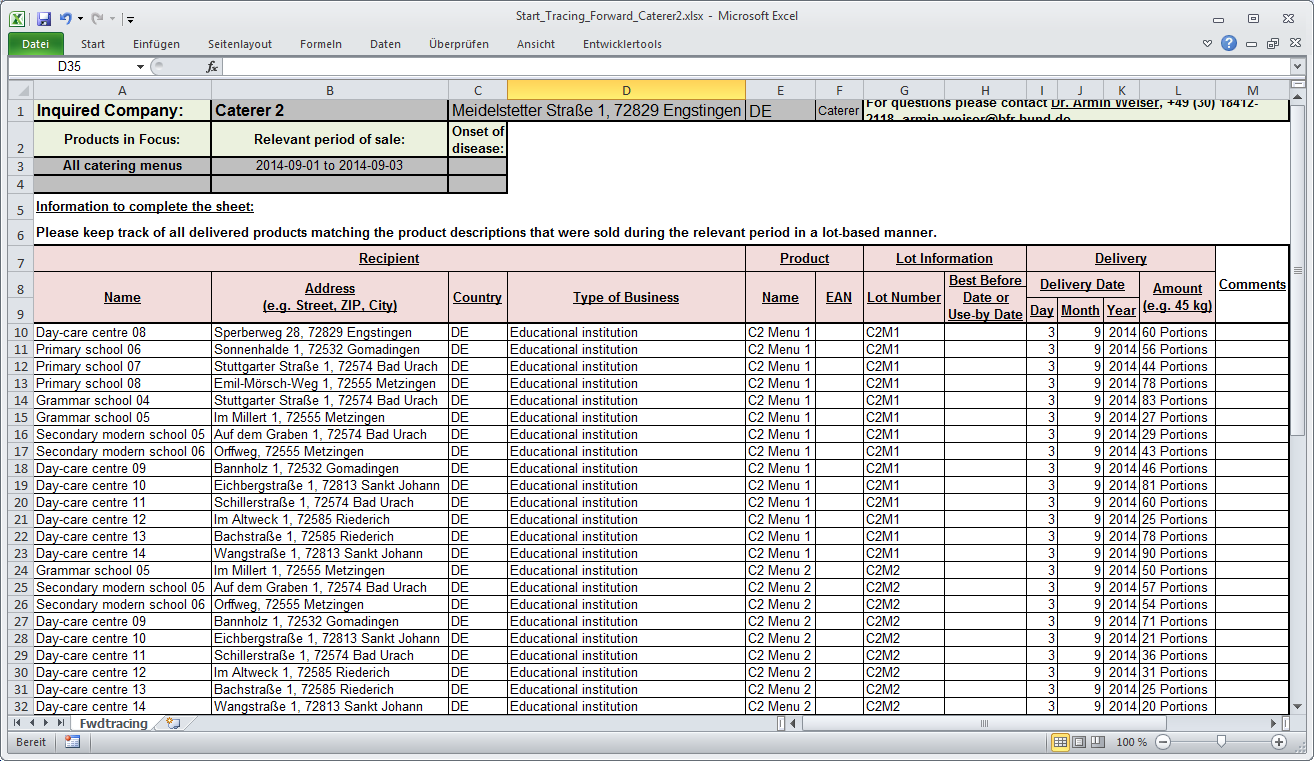
\includegraphics[height=0.55\textwidth]{4.png}
	\end{center}
	\begin{itemize}
		\item Download the pre-prepared templates.
		\item Caterer 1: \url{https://github.com/SiLeBAT/BfROpenLabResources/raw/master/GitHubPages/documents/Start_Tracing_Forward_Caterer1.xlsx}
		\item Caterer 2: \url{https://github.com/SiLeBAT/BfROpenLabResources/raw/master/GitHubPages/documents/Start_Tracing_Forward_Caterer2.xlsx}
	\end{itemize}
\end{frame}

\subsection{5}
\begin{frame}
	\begin{center}
  		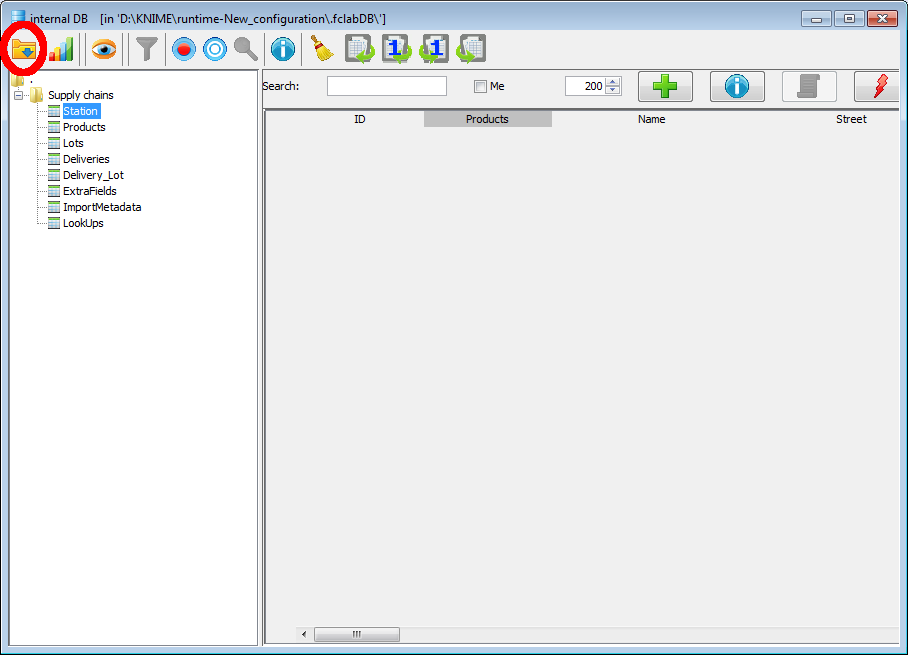
\includegraphics[height=0.6\textheight]{5.png}
	\end{center}
	\begin{itemize}
		\item To import the files click on the \textbf{Table import} button in the upper left corner of the database interface.
	\end{itemize}
\end{frame}

\subsection{6}
\begin{frame}
	\begin{center}
  		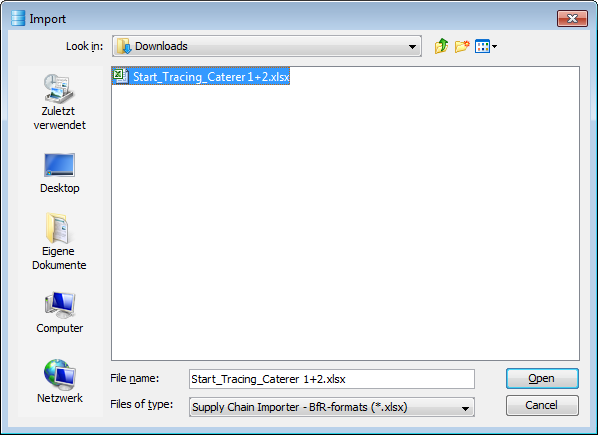
\includegraphics[height=0.5\textheight]{6.png}
	\end{center}
	\begin{itemize}
		\item In the file dialog that appears, select "Start\_Tracing\_Forward\_Caterer1.xlsx" and "Start\_Tracing\_Forward\_Caterer2.xlsx".
		\item Then press \textbf{Open}.
	\end{itemize}
\end{frame}

\subsection{7}
\begin{frame}
	\begin{center}
  		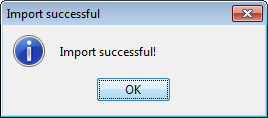
\includegraphics[width=0.4\textwidth]{7.png}
	\end{center}
	\begin{itemize}
		\item You'll see a message that the import was successful.
		\item Press \textbf{OK}.
	\end{itemize}
\end{frame}

\subsection{8}
\begin{frame}
	\begin{center}
  		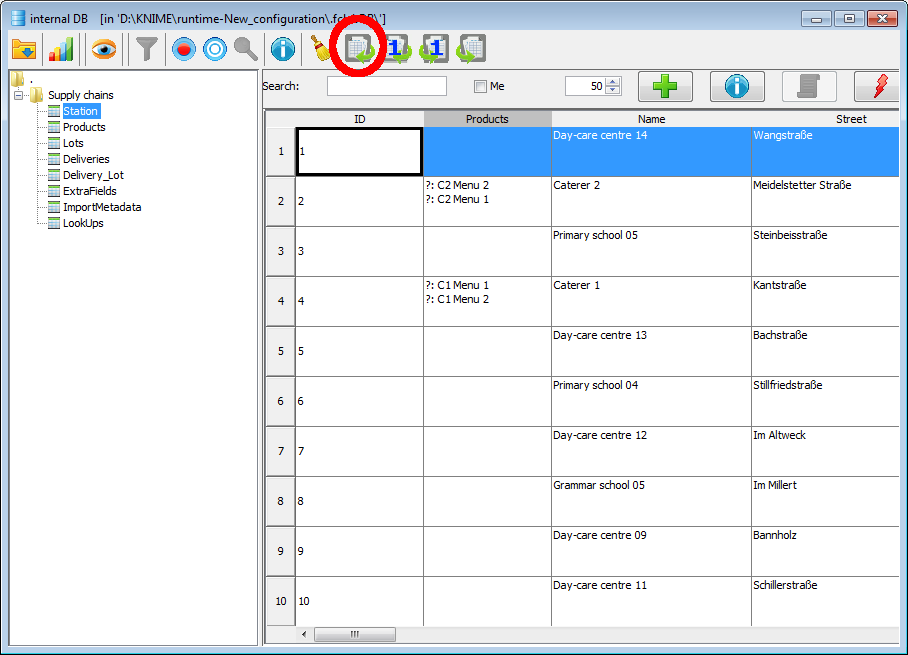
\includegraphics[height=0.5\textheight]{8.png}
	\end{center}
	\begin{itemize}
		\item In the database interface you'll notice, that there is now data in the tables.
		\item Now we want to do a backtracing starting from the caterers to see where they got the ingredient of the meals from.
		\item Press the button for generating backtracing templates, which is marked by the red circle.
	\end{itemize}
\end{frame}

\subsection{9}
\begin{frame}
	\begin{center}
  		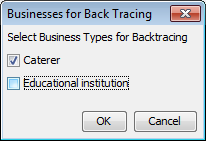
\includegraphics[width=0.4\textwidth]{9.png}
	\end{center}
	\begin{itemize}
		\item Since we want to do the backtracing for the caterers, select \textbf{Caterer} only and press \textbf{OK}.
	\end{itemize}
\end{frame}

\subsection{10}
\begin{frame}
	\begin{center}
  		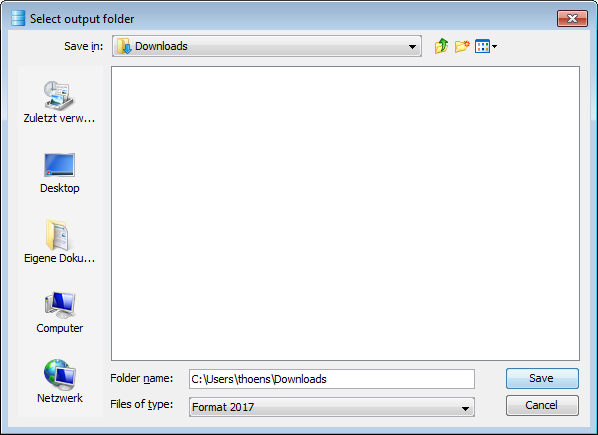
\includegraphics[height=0.5\textheight]{10.png}
	\end{center}
	\begin{itemize}
		\item In the file dialog that appears, you can specify the folder where the generated templates should be saved.
		\item Select or create the desired folder and press \textbf{Save}.
	\end{itemize}
\end{frame}

\subsection{11}
\begin{frame}
	\begin{center}
  		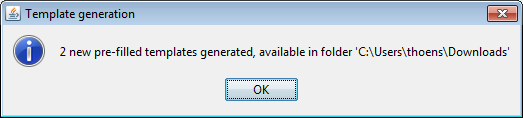
\includegraphics[width=0.8\textwidth]{11.png}
	\end{center}
	\begin{itemize}
		\item You'll be noticed, that 2 templates were generated in the folder you specified.
		\item Press \textbf{OK}.
	\end{itemize}
\end{frame}

\subsection{12}
\begin{frame}
	\begin{center}
  		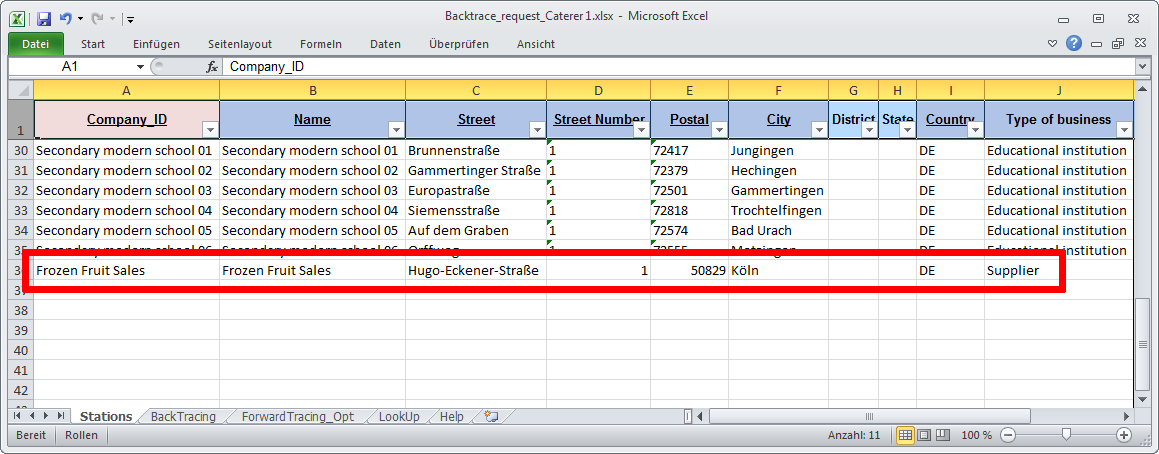
\includegraphics[height=0.55\textwidth]{12.png}
	\end{center}
	\begin{itemize}
		\item Open the generated template for "Caterer 1".
		\item In the upper part of the sheet you can see all the outgoing deliveries of "Caterer 1", that were imported with the "Start Forward Template". These deliveries belong to two different lots: "C1M1" and "C1M2".
		\item The cells here have grey background. That means that you should not edit them.
	\end{itemize}
\end{frame}

\subsection{13}
\begin{frame}
	\begin{center}
  		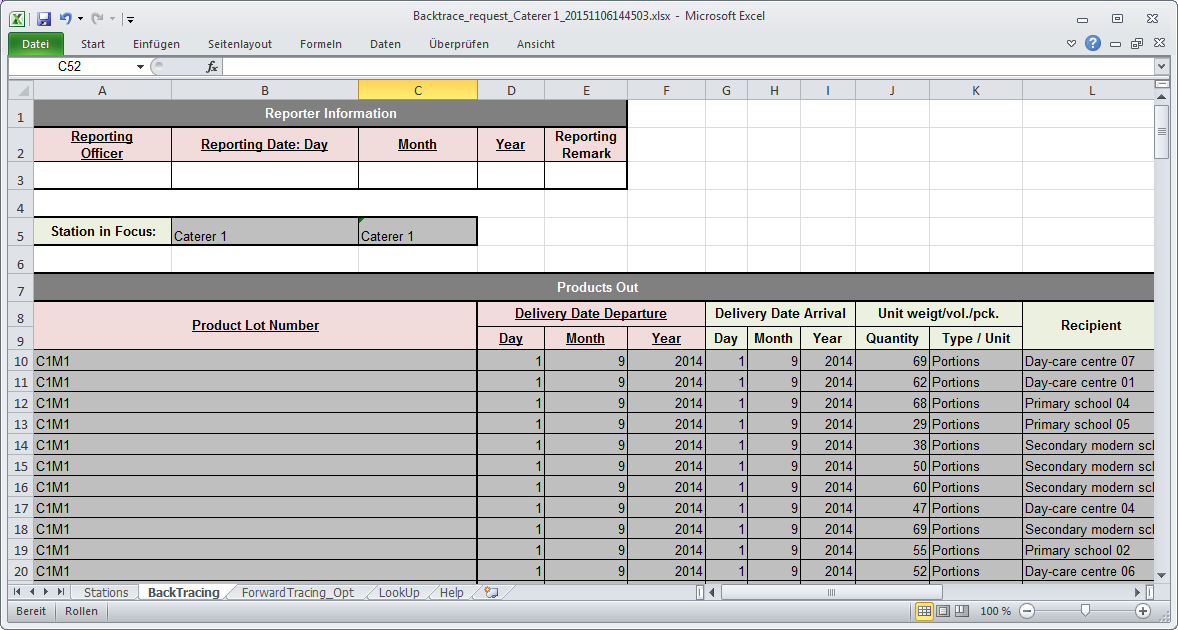
\includegraphics[height=0.5\textwidth]{13.png}
	\end{center}
	\begin{itemize}
		\item Scroll down to the section where you can enter the ingredient for the two lots.
		\item A delivery of "Frozen Strawberries" from "Frozen Fruit Sales" was used as an ingredient in lot "C1M1".
		\item So lets enter this delivery here (marked by the red box).
		\item Save and close the document.
	\end{itemize}
\end{frame}

\subsection{14}
\begin{frame}
	\begin{center}
  		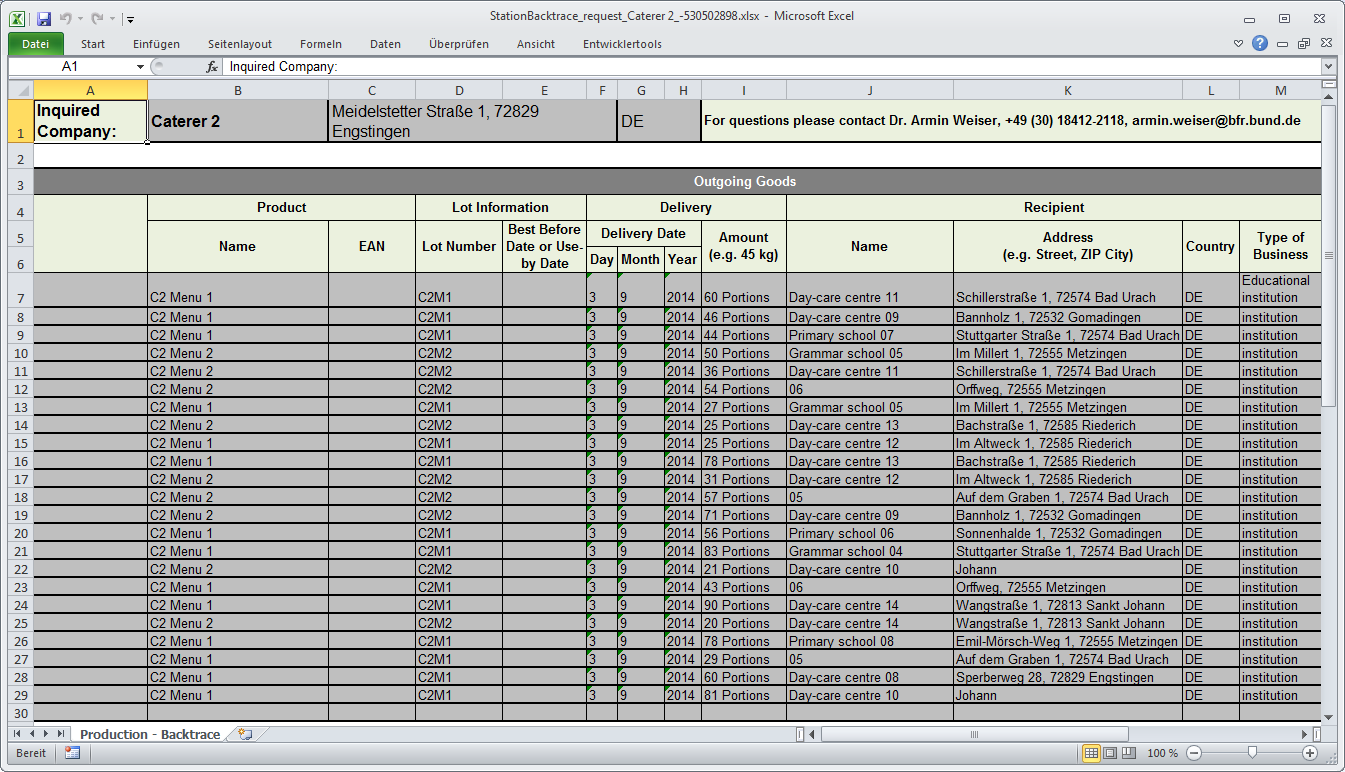
\includegraphics[width=0.8\textwidth]{14.png}
	\end{center}
	\begin{itemize}
		\item Now open the generated template for "Caterer 2".
		\item Analogously to the previous template you can see all the outgoing deliveries of "Caterer 2".
	\end{itemize}
\end{frame}

\subsection{15}
\begin{frame}
	\begin{center}
 		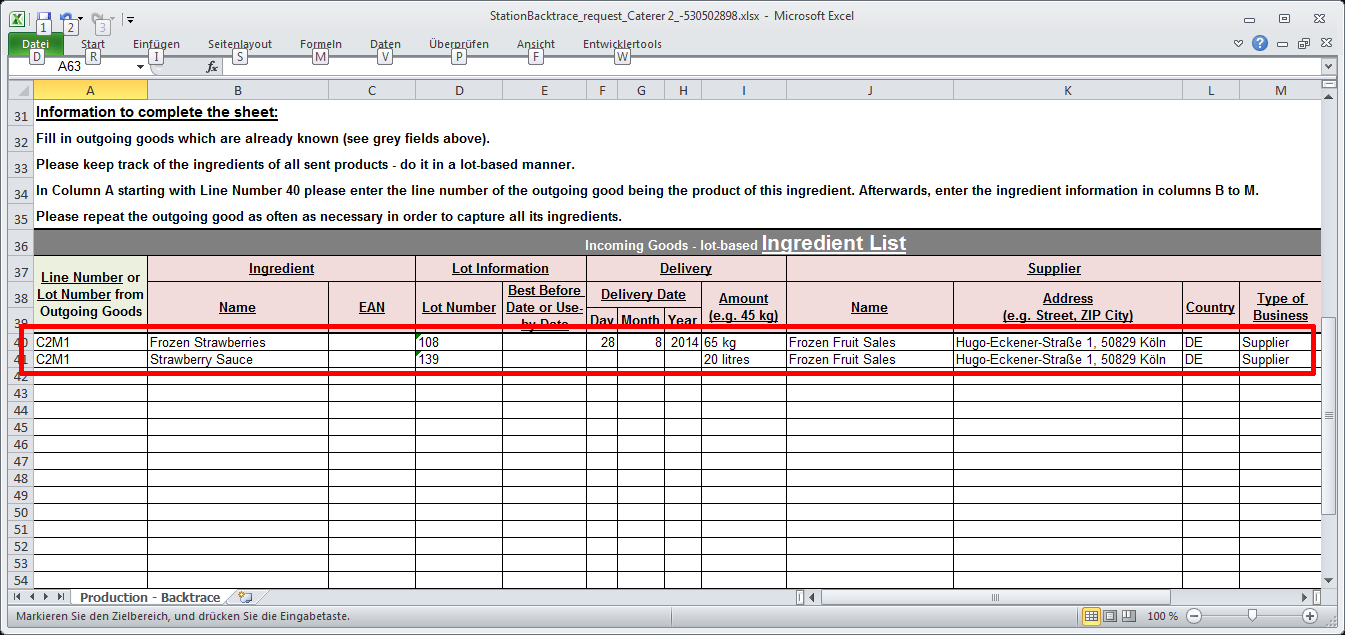
\includegraphics[width=0.95\textwidth]{15.png}
	\end{center}
	\begin{itemize}
		\item Scroll down to the section where you can enter the ingredient for the two lots.
		\item Two deliveries of strawberry products from "Frozen Fruit Sales" were used as ingredients in lot "C2M1".
		\item Enter the deliveries here (marked by the red box).
		\item Then save and close the document.
	\end{itemize}
\end{frame}

\subsection{16}
\begin{frame}
	\begin{center}
  		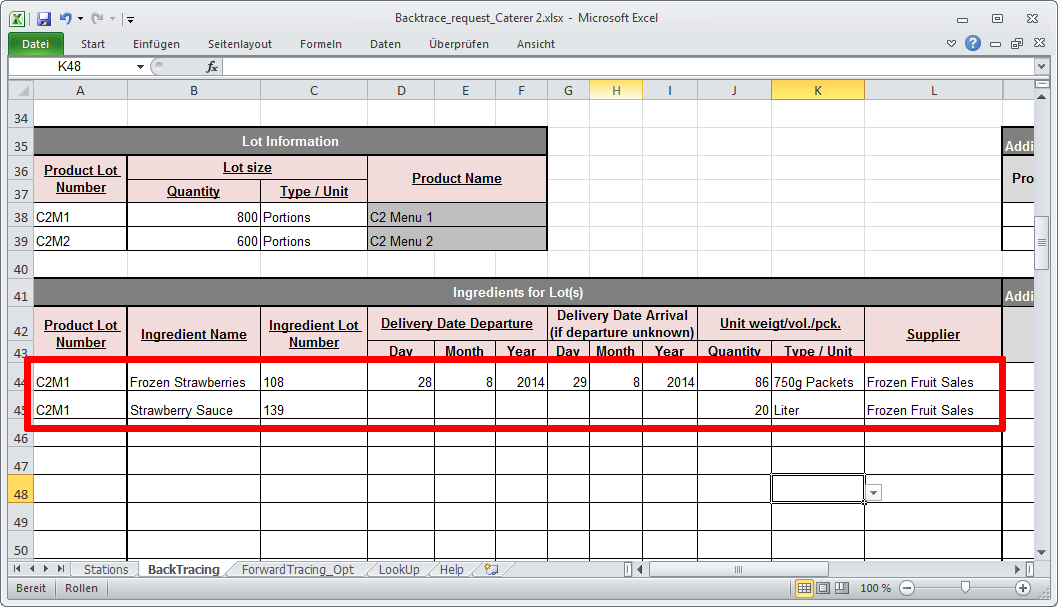
\includegraphics[width=0.95\textwidth]{16.png}
	\end{center}
	\begin{itemize}
		\item To import the two files into the database click on the \textbf{Table import} button in the upper left corner of the database interface.
	\end{itemize}
\end{frame}

\subsection{17}
\begin{frame}
	\begin{center}
  		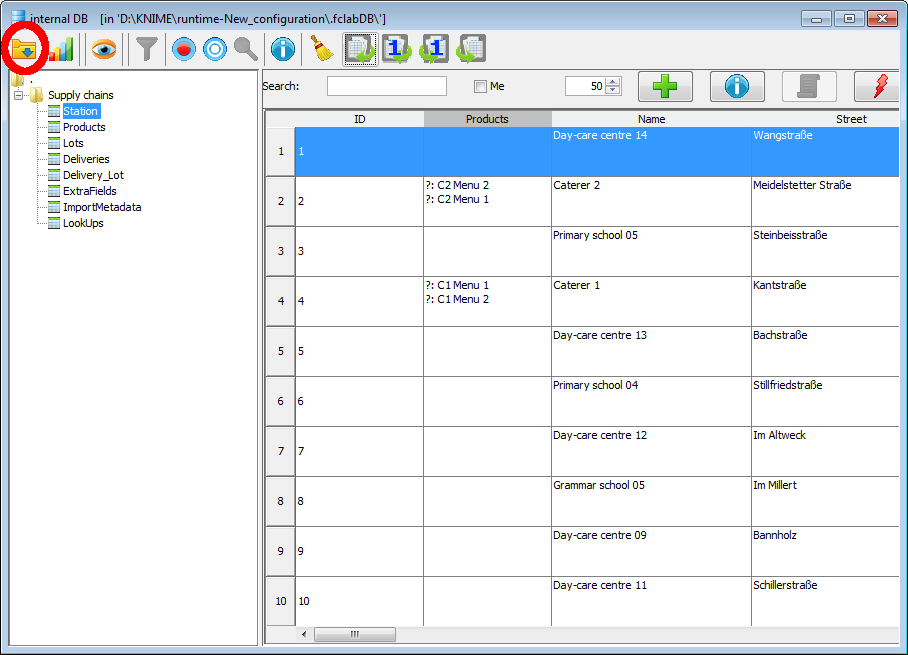
\includegraphics[height=0.6\textheight]{17.png}
	\end{center}
	\begin{itemize}
		\item In the file dialog that appears, select both backtracing templates.
		\item Then press \textbf{Open}.
	\end{itemize}
\end{frame}

\subsection{18}
\begin{frame}
	\begin{center}
  		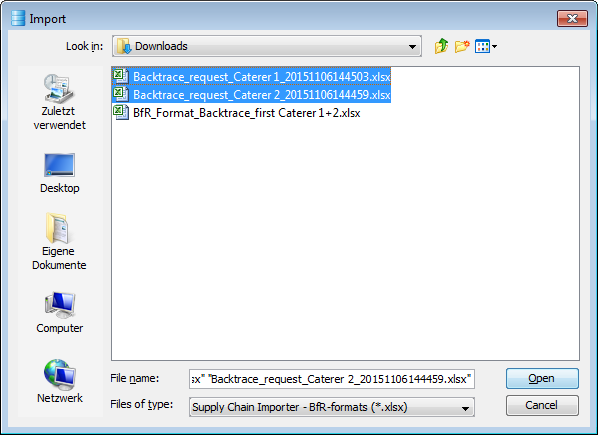
\includegraphics[height=0.2\textheight]{18.png}
	\end{center}
	\begin{itemize}
		\item You'll see a message that the import was successful.
		\item Press \textbf{OK}.
	\end{itemize}
\end{frame}

\end{document}